\documentclass[11pt,a4paper]{article}
\usepackage[utf8]{inputenc}
\usepackage[spanish]{babel}
\usepackage{amsmath}
\usepackage{amsfonts}
\usepackage{amssymb}
\usepackage{graphicx}
\usepackage[left=2cm,right=2cm,top=2cm,bottom=2cm]{geometry}
\title{Universidad Politécnica de la Zona Metropolitana de Guadalajara}
\begin{document}

\maketitle

\begin{figure}[h]
\begin{center}

\includegraphics[scale=1]{1.jpeg}
\end{center}
\end{figure}

\begin{center}
\author{Sistemas Electrónicos de Interfaz\\
Barrera Vazquez Omar\\
Ing.Mecatrónica 4B}
\end{center}

\newpage

\section{Objetivo de la practica}

El alumno sera capaz de reconocer los bloques que conforman la fuentes de alimentación conmutables, realizando simulaciones y diagrama de una fuente de alimentación regulable, esto para sus proyectos.

\section{Materiales}

Los materiales son los siguientes:

\begin{itemize}
\item transformador de 120V-12V
\item clavija con cable para el transformador
\item TRIAC BT137
\item DIAC 30V
\item capacitor poliester 100nF
\item 1 resistencia de 1k$\Omega$
\item 1 potenciómetro de 500K$\Omega$
\item 4 diodos rectificadores 1N4007
\item 3 capacitores de 100uF a 16 V
\item 1 timmer NE555
\item 2 capacitores cerámicos de 100pF
\item 1 bobina igual o mayor a 100uH
\item 1 diodo rectificador UF4003 0 4004
\item 1 potenciómetro 1k$\Omega$
\item 1 capacitor electrolítico de 2.2uF
\end{itemize}

\section{Desarrollo}

Básicamente en esta practica es la aplicación de conocimientos anteriores que se obtuvieron de la clase de electrónica de potencia, en la cual consistirá en armar una vuelve de voltaje regulable tipo \emph{buck, boots} desde que obtiene una entrada de voltaje de 120V de señal senoidal, esto para convertirla a una fuente de 3.3V en corriente directa e incluso se pueda regular.

En la siguiente imagen se observa como se tiene previsto el armado de la fuente alimentación, observe la figura 1:

\begin{figure}
\begin{center}
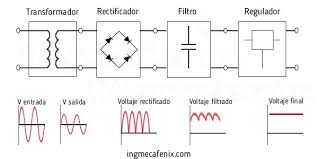
\includegraphics[scale=1]{2.jpeg}
\caption{bloques de una fuente de alimentación}
\end{center}
\end{figure}


\section{Transformador}

La función del transformador en la de convertir una señal senoidal de 127Vpp a 12Vpp una salida mas pequeña, sin tener que sacrificar la eficiencia, es por eso que el uso de los transformadores en fuentes de alimentación es de los mas usados. Este normalmente consta de dos embonados como se observa en la imagen 2:

\begin{figure}[h]
\begin{center}
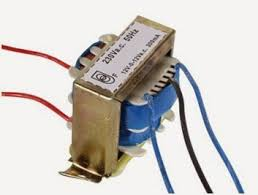
\includegraphics[scale=0.5]{3.jpeg}
\caption{embobinado de un transformador}
\end{center}
\end{figure}


\section{Regulador de intensidad}

En practicas anteriores se realizo un circuito que regulaba intensidad de una bombilla, este mismo sera utilizado para el circuito, antes de entrar al área o bloque de rectificación esto en caso de que queramos tener una intensidad mas controlada, para este bloque no es necesario entrar en detalles.

\section{Área de rectificación de onda}

Es aquí donde la onda se convierte de una onda senoidal completa con ciclos negativos y positivos, a una señal de media onda donde se aprecio la perdida de media onda. Se puede observar en la imagen 3 un puente de diodos rectificadores:

\begin{figure}[h]
\begin{center}
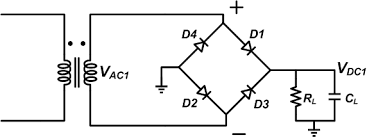
\includegraphics[scale=0.5]{4.jpeg}
\end{center}
\end{figure}

\section{Filtrado}

Prácticamente cuando la onda sale del área del rectificador, queda un rizado demasiado notable si lo vemos con un osciloscopio, su solución, poner de manera paralela capacitores que controles mas el rizado, pero eso no sera suficiente al momento de acercar mas con el osciloscopio, veremos que estos no desaparecen del todo, es aquí donde nos enfocamos con el regulador de tension tipo buck.

\begin{figure}[h]
\begin{center}
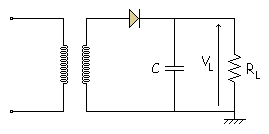
\includegraphics[scale=0.5]{5.png}
\end{center}
\end{figure}

\section{Regulador de voltaje}

Lo que hace un regulador de voltaje, nos ayuda desvanecer por completo o casi en su totalidad el rizado que deja el área o bloque de filtrado, por lo que también nos puede ayudar a variar la tension. Abajo se observa el diagrama de un regulador de voltaje y su esquema para la simulación en el software Kicad:

\begin{figure}
\begin{center}
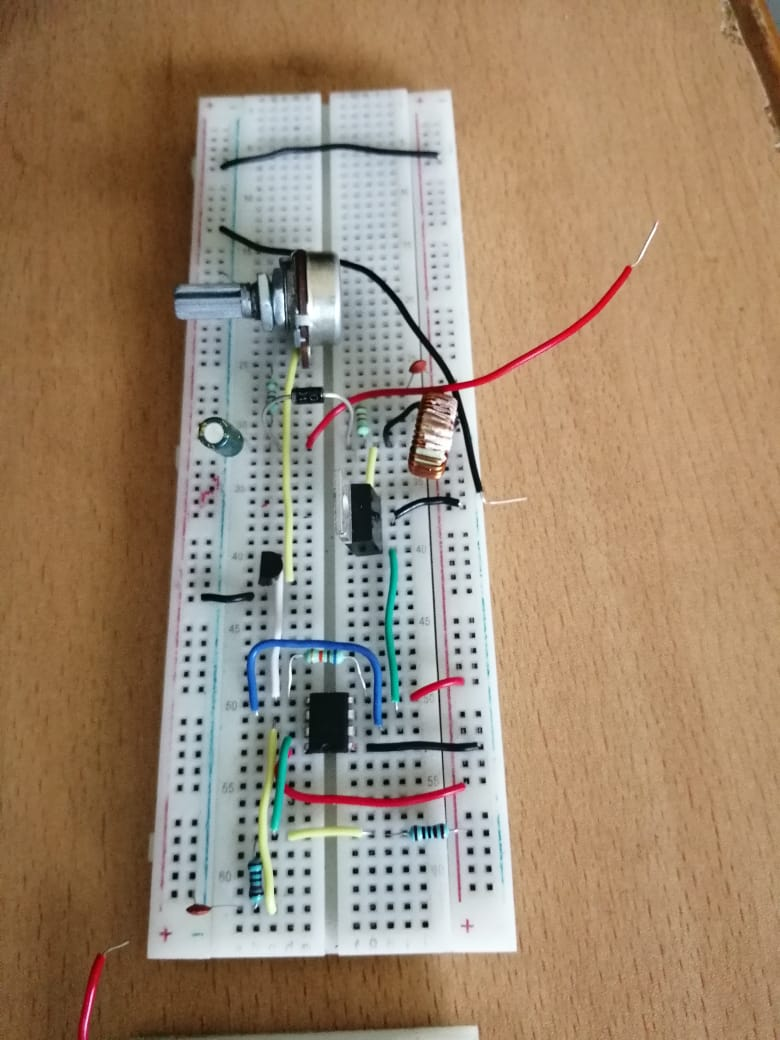
\includegraphics[scale=0.5]{6.jpeg}
\end{center}
\end{figure}



\section{conclusión}

Esta practica fue de suma importancia para la adquisición de conomiento sobre fuentes, ya que ayudo en el conocimiento de términos como los bloques de las fuentes de alimentación. Otra parte de lo aprendido fue el uso correcto de los transformadores y bobinas en circuitos AC y DC.

\end{document}